% fig_knapsack_interdiction: a toy knapsack interdiction instance.
% 8 items (box width = follower weight w, number = profit p), capacity C = 11,
% the leader may remove 2 items.  Data (checked by brute force over all 28
% removals and every follower packing):
%   w = 6 4 2 6 2 4 3 4,  p = 5 8 4 6 3 4 6 5,  C = 11.
%   No removal: follower packs value 21 (items 2,3,5,7, 1-based).
%   Best removal: items 2 and 7 (w 4, p 8 and w 3, p 6); the follower's best
%   packing of what is left is worth 13 (items 3,4,5: w 2+6+2 = 10, p 4+6+3);
%   the packing 3,6,8 ties at 13.  No other pair of removals gives 13 or less.
% Build: pdflatex fig_knapsack_interdiction.tex   (6.5 in x 1.8 in)
\documentclass[tikz,border=2pt]{standalone}
\usepackage{mathptmx}
\usetikzlibrary{arrows.meta,calc}
\definecolor{leader}{HTML}{2A78D6}
\definecolor{follower}{HTML}{EB6834}
\definecolor{cert}{HTML}{1BAF7A}
\definecolor{ink}{HTML}{0B0B0B}
\definecolor{ink2}{HTML}{52514E}
\definecolor{muted}{HTML}{A9A8A2}
\definecolor{grid}{HTML}{E6E5E0}
\tikzset{
  every picture/.style={font=\fontsize{8}{9.6}\selectfont, color=ink, line cap=round},
}
% \item{left}{width}{profit}{style}: one item box on the top row
\newcommand{\itembox}[4]{%
  \ifcase#4
    % 0: survives, not packed
    \draw[ink2, line width=0.6pt, fill=white] (#1,\ylo) rectangle ++(#2,\h);
    \node at ($(#1,\ylo)+(#2/2,\h/2)$) {#3};
  \or
    % 1: removed by the leader (grey with a cross)
    \draw[muted, line width=0.6pt, fill=grid] (#1,\ylo) rectangle ++(#2,\h);
    \draw[ink2, line width=0.9pt] (#1+0.08,\ylo+0.08) -- (#1+#2-0.08,\ylo+\h-0.08)
                                  (#1+0.08,\ylo+\h-0.08) -- (#1+#2-0.08,\ylo+0.08);
    \node[text=ink2, fill=grid, inner sep=1.2pt] at ($(#1,\ylo)+(#2/2,\h/2)$) {#3};
  \or
    % 2: survives and is packed by the follower
    \draw[follower, line width=0.8pt, fill=follower!22] (#1,\ylo) rectangle ++(#2,\h);
    \node at ($(#1,\ylo)+(#2/2,\h/2)$) {#3};
  \fi}
\begin{document}
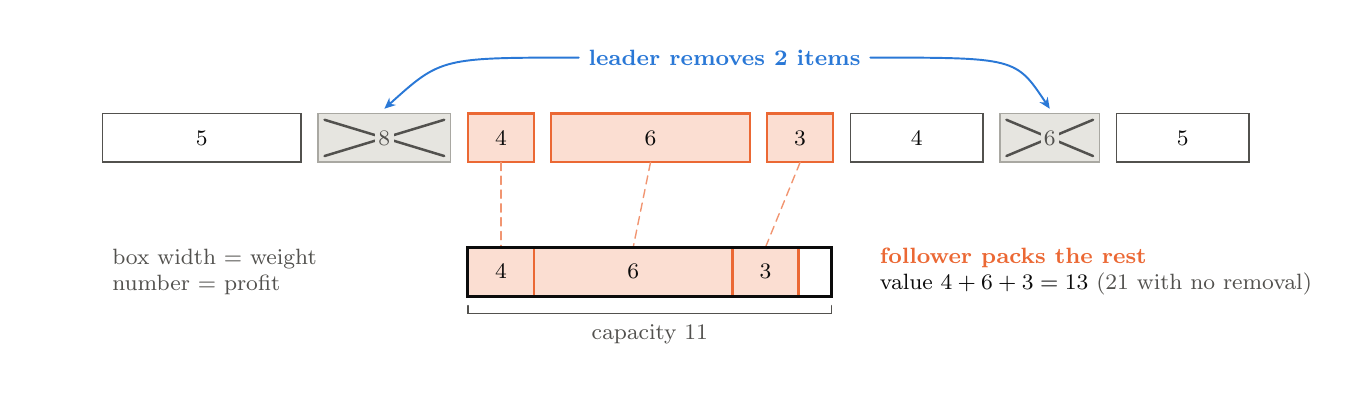
\begin{tikzpicture}
  % fixed page: 6.5 in x 1.8 in including the 2 pt border
  \useasboundingbox (0,0) rectangle (16.37,4.43);
  \begin{scope}[xshift=0.65cm] % centre the item row on the page
  \def\u{0.42}   % cm per unit of weight
  \def\h{0.62}   % box height
  \def\ylo{2.72} % bottom of the item row

  % ---- the 8 items (left x, width = w * u, profit, state) ----
  \itembox{0.30}{2.52}{5}{0}
  \itembox{3.04}{1.68}{8}{1}
  \itembox{4.94}{0.84}{4}{2}
  \itembox{6.00}{2.52}{6}{2}
  \itembox{8.74}{0.84}{3}{2}
  \itembox{9.80}{1.68}{4}{0}
  \itembox{11.70}{1.26}{6}{1}
  \itembox{13.18}{1.68}{5}{0}

  % ---- leader: removes 2 items ----
  \node[text=leader, font=\fontsize{8}{9.6}\selectfont\bfseries] (lead) at (8.20,4.05)
    {leader removes 2 items};
  \draw[leader, line width=0.7pt, -{Stealth[length=4pt,width=3.5pt]}]
    (lead.west) .. controls (4.6,4.05) .. (3.88,\ylo+\h+0.06);
  \draw[leader, line width=0.7pt, -{Stealth[length=4pt,width=3.5pt]}]
    (lead.east) .. controls (11.9,4.05) .. (12.33,\ylo+\h+0.06);

  % ---- follower: knapsack of capacity 11, packs the rest ----
  \def\yb{1.02}
  \foreach \from/\to/\w/\p in {4.94/4.94/0.84/4, 6.00/5.78/2.52/6, 8.74/8.30/0.84/3}{
    \draw[follower!70, line width=0.5pt, densely dashed]
      (\from+\w/2,\ylo) -- (\to+\w/2,\yb+\h);
    \draw[follower, line width=0.8pt, fill=follower!22] (\to,\yb) rectangle ++(\w,\h);
    \node at (\to+\w/2,\yb+\h/2) {\p};
  }
  % the knapsack outline: capacity 11 units
  \draw[ink, line width=1.1pt] (4.94,\yb) rectangle ++(11*\u,\h);
  \draw[ink2, line width=0.5pt] (4.94,\yb-0.12) -- ++(0,-0.1) -- ++(11*\u,0) -- ++(0,0.1);
  \node[text=ink2, anchor=north] at (4.94+5.5*\u,\yb-0.24) {capacity 11};
  \node[anchor=west, align=left] at (10.05,\yb+\h/2)
    {{\bfseries\color{follower}follower packs the rest}\\
     value $4+6+3 = 13$ \textcolor{ink2}{(21 with no removal)}};

  % ---- key ----
  \node[anchor=west, text=ink2, align=left] at (0.30,\yb+\h/2)
    {box width = weight\\ number = profit};
  \end{scope}
\end{tikzpicture}
\end{document}
